
\newcommand{\kLCS}{\textsf{LCS with $k$ Mismatches}}
\newcommand{\kApproxLCS}{\textsf{LCS with Approximately $k$ Mismatches}}
\newcommand{\acs}{\mathrm{ACS}}
\newcommand{\lcpk}{\mathrm{LCP}_{k}}
\newcommand{\lcpe}{\mathrm{LCP}_{(1+\eps)k}}
\newcommand{\Projections}{\Pi}
\newcommand{\Hashes}{\mathcal{H}}
\newcommand{\Collisions}{C}
\newcommand{\HD}{d_H}
\newcommand{\sk}{\mathrm{sk}}
\newcommand{\norm}[1]{\ensuremath{\lVert#1\rVert}}
\newcommand{\Ham}{\mathrm{Ham}}


\subsection{LCS(ubstring) with Approximately k Mismatches}
\begin{frame}
  \centering
  \beamermathcolor{black}
  {\Large The Longest Common Substring with Approximately $k$ Mismatches}
  
  \medskip
  {\large CPM'20}
  \bigskip

  
\includegraphics{pictures/mindmap/lcsk.png}

  \bigskip
  Tomasz Kociumaka, Jakub Radoszewski, Tatiana Starikovskaya
\end{frame}

\frame{
\frametitle{Similarity measures}

\textbf{Problem:} Given two strings $X$ and $Y$, How similar are they? 
\pause

\vspace*{0.2cm}
Ideally, something \textbf{Fast} and \textbf{Robust}:
\begin{itemize}
	\pause
	\item Strongly subquadratic time
	\pause
	\item Small change in the input $\Rightarrow$ small change of the similarity measure
\end{itemize}

\pause
\vspace*{0.2cm}
Applications in \textbf{bioinformatics}, \textbf{search engines} and \textbf{detection of plagiarism}.
}


\frame{
\frametitle{The Edit distance}
A very relevant similarity measure for biological sequences.\\
You are allowed \textbf{Insertion}, \textbf{Deletion}, and \textbf{Substitution}.

\pause
\begin{center}
 EditDistance(GATTACAT, ATTACATT) = 2
\end{center} 
 
 \pause
 Unfortunately,
 
 \begin{block}{[Backurs and Indik'15]}
 The Edit distance can't be computed in strongly subquadratic time, unless SETH is false.
 \end{block}
 
\pause
\textbf{SETH} the Strong Exponential Time Hypothesis : 3-SAT cannot be solved in subexponential time in the worst case.\\
Commonly believed to be true.

}



\frame{
\frametitle{The Longest Common Substring problem}

\begin{block}{LCS}
\textbf{Input}: Two strings $X, Y$ of length $n$.\\
\textbf{Output}: The longest substring that occurs both in $X$ and $Y$.
\end{block}

Issue: It is not robust.
\pause
\begin{center}
$X=a^{2m+1}$ and $Y= a^{2m}b$ $\Rightarrow$ $LCS(X,Y)=2m$\\
\pause
$X=a^{m}ba^m$ and $Y= a^{2m}b$ $\Rightarrow$ $LCS(X,Y)=m$
\end{center}
\pause
Only one character changed, and the LCS has been divided by 2.
}


\frame{
\frametitle{The Longest Common Substring with $k$ mismatches}
\begin{block}{\kLCS}
\textbf{Input}: Two strings $X, Y$ of length $n$, an integer $k$.\\
\textbf{Output}: A substring of $X$ that occurs in $Y$ with at most $k$ mismatches.
\end{block}
\pause
However...
\begin{block}{[Kociumaka, Radoszweski, Starikovskaya'19]}
 There is a $k = \Theta (\log(n))$ such that $LCS_k$ can't be computed in strongly subquadratic time, unless SETH is false.
 \end{block}

}

\frame{
\frametitle{The Longest Common Substring with Approximately $k$ mismatches}
\begin{block}{$LCS_{\tilde{k}}$}
\textbf{Input}: Two strings $X, Y$ of length $n$, an integer $k$.\\
\textbf{Output}: A substring of $X$ of length at least $LCS_k$ that occurs in $Y$ with at most $(1+\eps) \cdot k$ mismatches.
\end{block}

\pause

\begin{block}{[Kociumaka, Radosweski, Starikovskaya'19]}
  $LCS_{\tilde{k}}$ can be solved for $\eps < 2$, in $\Oh(n^{1+1/(1+\eps)}\log^2 n)$ time and $\Oh(n^{1+1/(1+\eps)})$ space.
\end{block}

}

\frame{
\frametitle{Our contributions}
\begin{myalertblock}{Upper bounds}{}{bg=Red,fg=white}
 Let $\eps > 0$ be an arbitrary constant. The \kApproxLCS problem can be solved correctly with high probability 
\begin{enumerate}[1)]
\item in $\Oh(n^{1+ 1/(1+2\eps) + o(1)} \log^2 n)$ time and $\Oh(n^{1+ 1/(1+2\eps) + o(1)})$ space assuming a constant-size alphabet;
\item and $\Oh(n^{1+1/(1+\eps)} \log^3 n)$ time and $\Oh(n)$ space for alphabets of arbitrary size. 
\end{enumerate}
\end{myalertblock}

\pause

\begin{myalertblock}{Lower Bound}{}{bg=Red,fg=white}
Assuming SETH, for every constant $\delta > 0$, there exists a constant $\eps = \eps(\delta)$ such that given $X$ and $Y$ of size $n$ computing the \kApproxLCS requires $\Omega(n^{2-\delta})$ time. 
\end{myalertblock}
}


\frame{
\frametitle{Twenty question game with a liar}

\begin{center}
\hspace{0.1\textwidth}
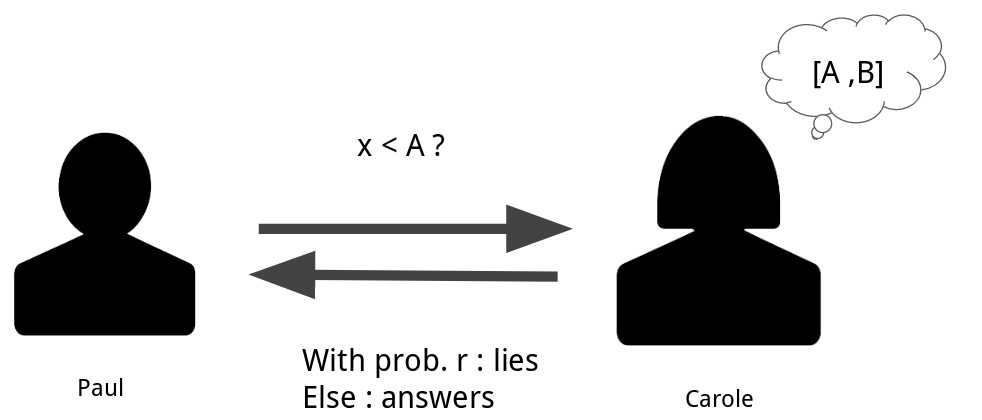
\includegraphics[width=0.8\textwidth]{figures/20q}
\end{center}

\begin{block}{[Dhagat, G{\'a}cs, Winkler '92]}
For $A = B$, Paul has a winning strategy for all $r < \frac{1}{3}$ asking $Q = \lceil \frac{8 \log N}{(1-3r)^2} \rceil =  \Theta(\log n)$ questions.
\end{block}

}

\frame{
\frametitle{Decision variant }

\btheme{Input:} integers ${k, \ell}$, a constant ${\eps > 0}$, strings ${S_1, S_2}$ of length ${n}$

\btheme{Output:} 

\begin{enumerate}
\item YES if ${\ell \le \mathrm{LCS_k}}$;
\item YES or NO if ${\mathrm{LCS_k} < \ell \le \mathrm{LCS_{(1+\eps)k}}}$; 
\item NO if ${\mathrm{LCS_{(1+\eps)k}} < \ell}$.
\end{enumerate}

The answer must be correct with probability at least $3/4$.

\pause
\par\noindent\ntheme{\rule{\textwidth}{1pt}}

\ntheme{Longest Common Substring with approx. $k$ mismatches:}

\medskip
\begin{itemize}
\item $A = \mathrm{LCS_k}$ and $B = \mathrm{LCS_{(1+\eps)k}}$.\\
\item An algorithm for the decision variant plays the role of Carole. \\
\item With ${\lceil \frac{8 \log n}{(1-3r)^2} \rceil}$ questions, Paul will find $x \in [\mathrm{LCS_k}, \mathrm{LCS_{(1+\eps)k}}]$ for some $1/4 < r < 1/3$.
\end{itemize}

}


\frame{
\frametitle{Locality-Sensitive Hashing}
Nearest Neighbour search, data clustering...\\
In string processing: Andoni and Indyk for a space-efficient randomized index for approximate pattern matching.
\pause
\begin{enumerate}
\item Projections:
\vspace{-0.5cm}
$$h(S)=S[a_{p_1}] S[a_{p_2}] \cdots S[a_{p_m}]$$
And Collisions-Sets (Karp-Rabin fingerprints).
$$\Collisions^{\Hashes}_{\ell} = \{(S_1,S_2, h) :\varphi(h(S_1 0^{n-\ell})) = \varphi(h(S_2 0^{n-\ell})) \}$$
\pause
\item Dimension reduction.
\vspace{0.1cm}
With probability at least $1- n^{-\beta}$, for all $u,v \in P$:\\
\begin{enumerate}[1)]
\item if $\norm{\sk_\alpha(u)-\sk_\alpha(v)}^2 \le (1+\alpha) \cdot k$, then $\HD(u,v) \le (1+\alpha) \cdot k$;
\item if $\norm{\sk_\alpha(u)-\sk_\alpha(v)}^2 > (1+\alpha) \cdot k$, then $\HD(u,v) \ge k$.
\end{enumerate}
\end{enumerate}
}



\frame{
\frametitle{Algorithm}

\begin{algorithm}[H]
\small
%\caption{LCS with approx. $k$ mismatches, decision variant}
\begin{algorithmic}[1]
\State Choose a set $\ntheme{\Hashes}$ of ${\Theta(n^{1/(1+\eps)})}$ functions from ${\Projections^m}$ u.a.r.
\State $\ntheme{\Collisions^{\Hashes}_{l} :=}$ set of all collisions of $l$-length substrings of $\ntheme{S_1, S_2}$ under the hash functions in $\ntheme{\Hashes}$
\State Draw a collision $\ntheme{(X, Y) \in \Collisions^{\Hashes}_{\ell}}$ uniformly at random 
\If {$\ntheme{\Ham (X, Y) \le (1+\eps) \cdot k}$}
	\Return YES
\EndIf
\State Choose a subset $\ntheme{\Collisions' \subseteq \Collisions^{\Hashes}_{l}}$ of size $\ntheme{\min\{\Collisions^{\Hashes}_{\ell}, 4nL\}}$
\For {$\ntheme{(X, Y) \in \Collisions'}$} 
	\If {$\ntheme{\Ham(S_1, S_2) \le k}$} 
		\Return YES
	\EndIf
\EndFor
\State \Return NO
\end{algorithmic}
\end{algorithm}

\pause
\ntheme{Running time $\Oh(n^{1+1/(1+\eps)} \log n)$:}
\begin{enumerate}
\item Compute the hash values and $\Collisions'$: $\Oh(n^{1+1/(1+\eps)} \log n)$ time (FFT)

\item Pick a random collision: $\Oh(n^{1+1/(1+\eps)})$ time (reservoir sampling)

\item Test in line 5: $\Oh(n^{1+1/(1+\eps)} \log^2 n)$ time (dimension reduction)

\item Test in line 7: $\Oh(n)$ time (character-by-character)
\end{enumerate}
}

\frame{
\frametitle{Experiments}

None of the previous solutions have been implemented. 

The only algorithm that seemed to be practical enough is the dynamic programming one \ntheme{[Flouri et al.'15]}

\pause
\bigskip

We compared our algorithm with the dynamic programming one
\begin{itemize}
 \item On random strings;
 \item On strings extracted from E. coli.
\end{itemize}

\medskip

Lengths from $5000$ to $60000$, $k = 10, 25, 50$
}

\frame{
\frametitle{Adjustments to the theory}
Implemented in C++ available on github.
\begin{enumerate}

\item Sketching for the Hamming distance via dimension reduction: replaced by a naive comparison character by character, Bit parallelism.
\pause

\item Computation of the collisions: A naive implementation, FFT and NTT.
\pause

\item The twenty question game: the twenty question game, binary search.
\pause

\item The number of hash functions $L$: $L = n^{1/(1+\eps)}$, $L = n^{1/(1+\eps)}/\log(n)$.

\end{enumerate}

}




\frame{
\frametitle{Running time}


\begin{figure}[ht!]
\centering
    \begin{subfigure}{.5\textwidth}
        \centering
        \captionsetup{justification=centering}
        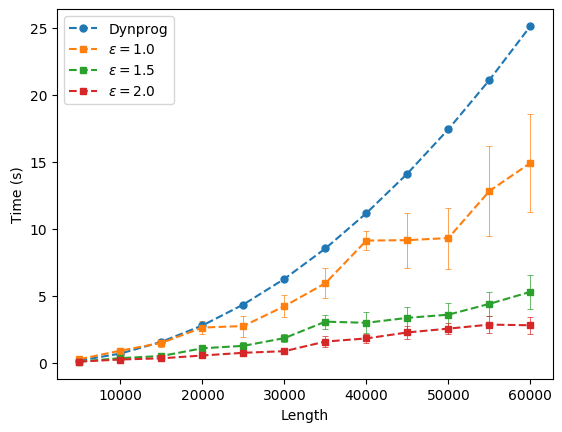
\includegraphics[scale=0.4]{figures/random_25.png}
        \caption{Random, $k = 25$}
    \end{subfigure}%
    \begin{subfigure}{0.5\textwidth}
        \centering
        \captionsetup{justification=centering}
        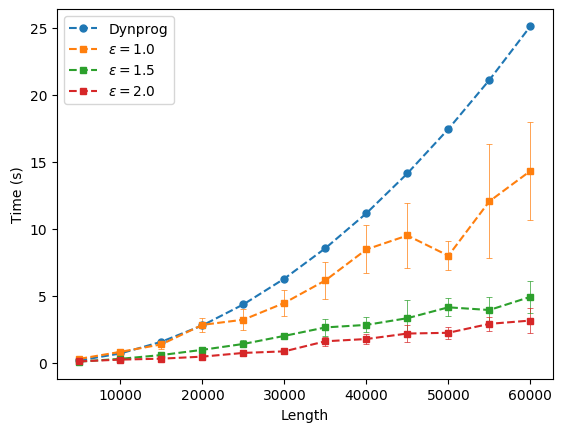
\includegraphics[scale=0.4]{figures/e_coli_25.png}
        \caption{E. coli, $k = 25$}
    \end{subfigure}     

\end{figure}


\bigskip

\begin{itemize}
\item For each length, we performed $10$ independent experiments
\item Big standard deviation for $\eps = 1$, negligible for $\eps = 1.5$ and $\eps = 2.0$
\item Gain up to a factor of 10 on strings of length $60000$
\end{itemize}
}



\frame{
\frametitle{Distortion and accuracy}

\begin{columns}
\column{0.5\textwidth}    
{\small
We estimate distortion by computing two values:

$r_{\min}(\eps, k) = \min_{S_1,S_2}(\mathrm{LCS_{\tilde{k}}}(S_1,S_2)/\mathrm{LCS_k}(S_1,S_2))$\\
$r_{\max}(\eps, k) = \max_{S_1,S_2}(\mathrm{LCS_{\tilde{k}}}(S_1,S_2)/\mathrm{LCS_k}(S_1,S_2))$

Furthermore, we can only err by returning a string shorter than $\mathrm{LCS_k}$.
}

\column{0.6\textwidth}

\newcolumntype{?}{!{\vrule width 1pt}}
\newcommand{\err}{\textcolor{red}{\mathrm{err}}}
\begin{center}
\begin{table}
\begin{tabular}{|l?l|l|l|l|l|l|}
\hline
 & \multicolumn{6}{c|}{\ntheme{Random}}\\ 
\hline
 & \multicolumn{2}{c|}{$\eps = 1.0$} & \multicolumn{2}{|c|}{$\eps = 1.5$} & \multicolumn{2}{|c|}{$\eps = 2.0$}\\ 
\hline

\multirow{ 2}{*}{$k = 10$} & 0.92 & 1.50 & 1.00 & 1.53 & 1.13 & 1.87\\ 
\cline{2-7}
& \multicolumn{2}{c|}{$\err = 7\%$}  & \multicolumn{2}{c|}{$\err = 0\%$}   & \multicolumn{2}{c|}{$\err = 0\%$}\\ 
\hline
\multirow{ 2}{*}{$k = 25$}  & 1.10 & 1.48 & 1.30 & 1.70 & 1.55 & 2.11\\ 
\cline{2-7}
& \multicolumn{2}{c|}{$\err = 0\%$}  & \multicolumn{2}{c|}{$\err = 0\%$}   & \multicolumn{2}{c|}{$\err = 0\%$}\\ 
\hline
\hline

& \multicolumn{6}{c|}{\ntheme{E. coli}} \\ 
\hline
& \multicolumn{2}{|c|}{$\eps = 1.0$} & \multicolumn{2}{c|}{$\eps = 1.5$} & \multicolumn{2}{c|}{$\eps = 2.0$} \\ 
\hline

\multirow{ 2}{*}{$k = 10$} & 0.86 & 1.41 & 0.91 & 1.47 & 0.95 & 1.71\\ 
\cline{2-7}
& \multicolumn{2}{|c|}{$\err = 34\%$}   & \multicolumn{2}{c|}{$\err = 13\%$}  & \multicolumn{2}{c|}{$\err = 8\%$}\\ 
\hline
\multirow{ 2}{*}{$k = 25$}  & 0.94  & 1.45 & 0.96 & 1.75 & 0.98 & 1.96\\ 
\cline{2-7}
& \multicolumn{2}{c|}{$\err = 7\%$}   & \multicolumn{2}{c|}{$\err = 5\%$}  & \multicolumn{2}{c|}{$\err = 2\%$}\\ 
\hline

\end{tabular} 
\label{tb:eps}
\end{table}
\end{center}


\end{columns}

}